%% The first command in your LaTeX source must be the \documentclass command.
%%
%% Options:
%% twocolumn : Two column layout.
%% hf: enable header and footer.
\documentclass[
twocolumn,
% hf,
]{ceurart}

%%
%% One can fix some overfulls
\sloppy

%%
%% Minted listings support 
%% Need pygment <http://pygments.org/> <http://pypi.python.org/pypi/Pygments>
\usepackage{listings}
%% auto break lines
\lstset{breaklines=true}

\usepackage{blindtext}
\usepackage[linesnumbered,ruled]{algorithm2e}
\usepackage{amsmath}
\usepackage{tikzsymbols}
\usepackage{pifont} % for \ding command
\usepackage{listings}
\usepackage{multirow}
\usepackage{bm}
\usepackage{bbm}
\usepackage{xfrac}
\usepackage{booktabs} % For better horizontal rules
\usepackage{cellspace} % For adjusting vertical spacing
\usepackage{xcolor}
\newcommand\todop[1]{\textcolor{red}{#1}} % todo in the paper
\newcommand\todos[1]{\textcolor{blue}{#1}} % todo in the software
\newcommand{\tik}{\textcolor{green}{\ding{51}}}
\newcommand{\ntik}{\textcolor{red}{\ding{55}}}
\usepackage{lastpage}
\usepackage{caption}
\usepackage{subcaption}

\newcommand{\xcc}{\mathbf{x_{/s}}}
\newcommand{\Xcal}{\mathcal{X}}
\newcommand{\xb}{\mathbf{x}}
\newcommand{\xc}{\mathbf{x_c}}
\newcommand{\Xc}{\mathbf{X_c}}
\newcommand{\xci}{\mathbf{x}^i_c}



%%
%% end of the preamble, start of the body of the document source.
\begin{document}

%%
%% Rights management information.
%% CC-BY is default license.
\copyrightyear{2024}
\copyrightclause{Use permitted under Creative Commons License Attribution 4.0 International (CC BY 4.0).}

%%
%% This command is for the conference information
\conference{The 2nd World Conference on eXplainable Artificial Intelligence,
  July 17--19, 2024, Malta, Valetta}

%%
%% The "title" command
\title{Fast and accurate regional effect plots for inspecting black-box models fit on tabular data}

%%
%% The "author" command and its associated commands are used to define
%% the authors and their affiliations.
\author[1,2]{Vasilis Gkolemis}
\address[1]{Harokopio University of Athens}
\address[2]{ATHENA Research Center}
\author[1]{Christos Diou}
\author[3]{Eirini Ntoutsi}
\address[3]{University of the Bundeswehr Munich}
\author[2]{Theodore Dalamagas}
\author[4]{Bernd Bischl}
\address[4]{Munich Center for Machine Learning (MCML), Department of Statistics, LMU Munich}
\author[4]{Julia Herbinger}
\author[4]{Giuseppe Casalicchio}


%%
%% The abstract is a short summary of the work to be presented in the
%% article.
\begin{abstract}
  Feature effect methods are a novel approach to extract insights from tabular data with the following procedure.  A black-box machine learning model is trained on a tabular dataset, a feature effect method explains its learnings, and the explanations (output of the feature effect method) are used to understand the data and and support decision making.  Feature effect methods can be global or regional. Regional effects have the benefit of automatically identifying important subgroups but in the cost of added complexity. Global effects provide one explanation per feature, for example, how age influences the annual income, while regional effects give separate explanations based on subgroups, for example, how age influences the annual income differently for men and women.  Existing regional effect methods suffer from efficiency and accuracy limitations. In this paper, we introduce rRHALE (regional RHALE), a method that overcomes these issues. rRHALE is notably more efficient, making it suitable for large datasets and complex models. It also handles correlated features effectively. We demonstrate its effectiveness with synthetic examples, comparing it to other feature effect methods, and apply rRHALE to a real-world scenario. The supporting code for this publication is available here.
\end{abstract}

%%
%% Keywords. The author(s) should pick words that accurately describe
%% the work being presented. Separate the keywords with commas.
\begin{keywords}
  Explainability \sep
  Interpretability \sep
  Feature Effect \sep
  Regional Effect \sep
  Global Explanations
\end{keywords}

%%
%% This command processes the author and affiliation and title
%% information and builds the first part of the formatted document.
\maketitle

\section{Introduction}
\label{sec:introduction}


% Recently, there has been a significant surge in the volume of available data.
% To harness the value of this data, there is a need for data analytics tools, i.e.,
% automated methods that provide insights on the available data.

There's been a significant increase in available data recently, prompting a need for data analytics tools to derive insights. Alongside this surge, Machine Learning methods have gained traction for their ability to automatically learn patterns and perform tasks like predictions. However, many Machine Learning models operate as black-boxes, meaning they take inputs and produce outputs without transparent inner workings. To address this, explainability techniques have emerged to shed light on these models' inner mechanisms.

A promising approach to understanding data involves using machine learning models and then explaining them, essentially using model understanding to achieve data understanding.



% The increasing adoption of machine learning (ML) in high-stakes domains like healthcare and finance has raised the demand
% for explainable AI (XAI) techniques~\citep{freiesleben_scientific_2022, ribeiro2016should}.
% Global feature effect methods explain a black-box model through a set of plots, where each plot is the effect of a feature on the output, as in Figure~\ref{subfig:a}.

% Global effects may be misleading when the black-box model $f(\cdot)$ exhibits interactions between features.
% An interaction between two features, $x_s$ and $x_k$,
% %EIRINI: xs, xk should be introduced properly Vasilis: Done!
% exists when the difference in the output $f(\mathbf{x})$ as a result of changing the value of $x_s$ \textit{depends} on the value of $x_k$~\citep{friedman_predictive_2008}.
% Global effects are often computed as averages over local effects.
% % For example, individual conditional expectation (ICE) curves~\citep{goldstein_peeking_2014} are the local counterparts of partial dependence plots (PDP) see also example in Fig.~\ref{fig:main-concept}.
% When feature interactions are present, local effects become heterogeneous, i.e., they significantly deviate from the average (global) effect.
% In these cases, the global effect may be misleading, a phenomenon known as \emph{aggregation bias}~\citep{mehrabi_survey_2021, herbinger_repid_2022}.

% Regional~\citep{herbinger2023decomposing, herbinger_repid_2022, molnar2023model, britton2019vine, hu2020surrogate, scholbeck2022marginal} or cohort explanations~\citep{sokol2020explainability}, partition the input space into subspaces and compute a regional explanation within each.
% The partitioning aims at subspaces with homogeneous local effects, i.e., with reduced feature interactions, yielding regional effects with minimized aggregation bias~\citep{herbinger_repid_2022}. 
% By combining these regional explanations, users can interpret the model's behavior across the entire input space.
% Several libraries focus on XAI, but
% none targets on regional effect methods (Table~\ref{tab:package-comparison}). Therefore, we present \texttt{Effector}, a Python library dedicated to regional explainability methods, which:

\begin{itemize}
\item implements well-established global and regional effect methods, accompanied by an intuitive way to visualize the heterogeneity of each plot. 
\item follows a consistent and modular software design. Existing methods share a common API and novel methods can be easily added and compared to existing ones.
\item demonstrates through tutorials the use of regional effects in real and synthetic datasets.
\end{itemize}

\begin{figure*}[t]
    \centering
    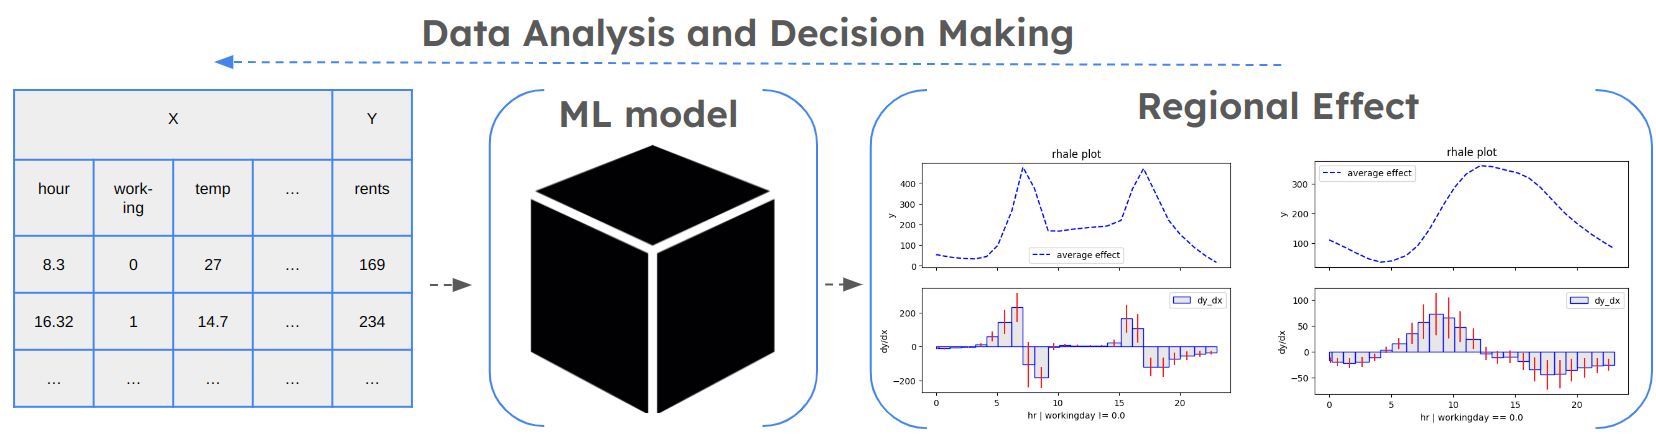
\includegraphics[width=\textwidth]{figures/concept_image.png}
    \caption{Data analysis and decision making pipeline: Utilizing regional effect plots to extract insights from tabular data.}
    \label{fig:concept_figure}
\end{figure*}


\section{Regional RHALE}



\subsection{Method Description}

\subsection{Computational Complexity}

All regional effect methods follow the CART-based approach of Algorithm(add reference), with computational complexity of ... Algorithm(cite) executes the prediction function $(D-1) \times N_2 $ for computing the best split on a particular level, leading to a total of $(D-1) \times N_2 \times M$ execution of f.


\section{Synthetic Example 1}

The purpose of this example is to shwocase the superiority of Regional RHALE compared to Regional PDP, when features are correlated. In such cases, Regional PDP may erroneously find subregions due to out of distribution sampling.

Consider a black-box function $y = 3x_1I_{x_3>0} - 3x_1I_{x_3\leq0} + x_3$ and two different setting for the data generating distribution. In the non-correlated setting, all variables are uniformly distributed, i.e., $x_i \sim \mathcal{U}(-1,1)$.
In the correlated setting, we keep the same distributions for $x_1$ and $x_2$, but we set $x_3 = x_1$. We will focus on the effect (global and regional) of $x_1$ on $y$.

\paragraph{Non-correlated setting.}

The effect of $x_1$ is provoked by the interaction terms, i.e., $3x_1I_{x_3>0}$ and $3x_1I_{x_3\leq0}$. The global effect will be $3x_1$ when $x_3>0$ (half of the times considering that $x_3 \sim \mathcal{U}(-1,1)$) and $-3x_1$ when $x_3 \leq 0$ (the other half). This results in a zero global effect with high heterogeneity. If splitting into two subregions, $x_3>0$ and $x_3 \leq 0$, we get two regional effects, $3x_1$ and $-3x_1$, with zero heterogeneity each. In figure~\ref{fig:synthetic-1-uncorrelated}, we observe that both rPDP and rRHALE find correctly both global and regional effect.




\begin{figure*}[t]
    \centering
    \begin{subfigure}[b]{0.33\textwidth}
        \centering
        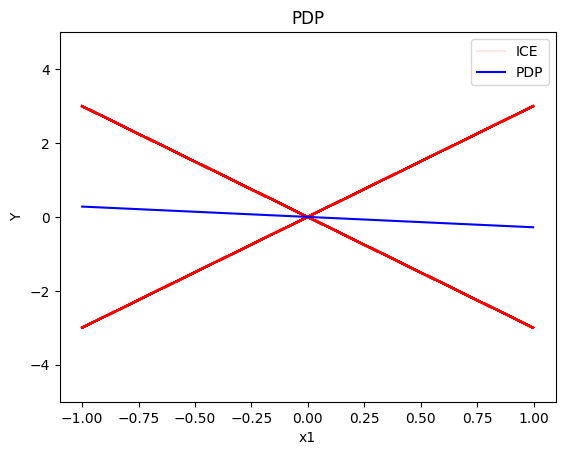
\includegraphics[width=\textwidth]{figures/simulation_1/uncor_global_pdp.png}
        \caption{Global PDP ($x_1$)}
        \label{subfig:a}
    \end{subfigure}
    \begin{subfigure}[b]{0.33\textwidth}
        \centering
        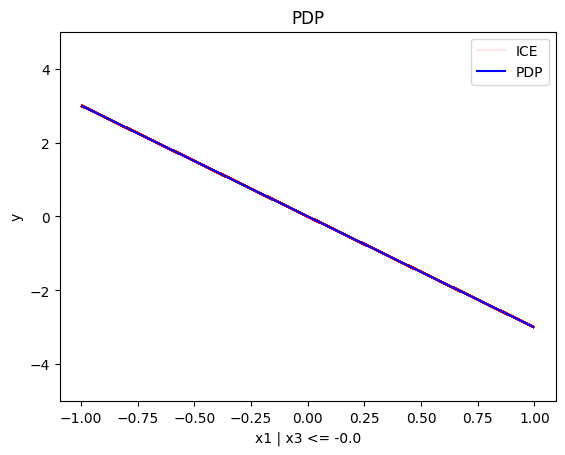
\includegraphics[width=\textwidth]{figures/simulation_1/uncor_regional_pdp_1.png}
        \caption{Regional PDP ($x_1 | x_3 \leq 0$)}
        \label{subfig:b}
    \end{subfigure}
    \begin{subfigure}[b]{0.33\textwidth}
        \centering
        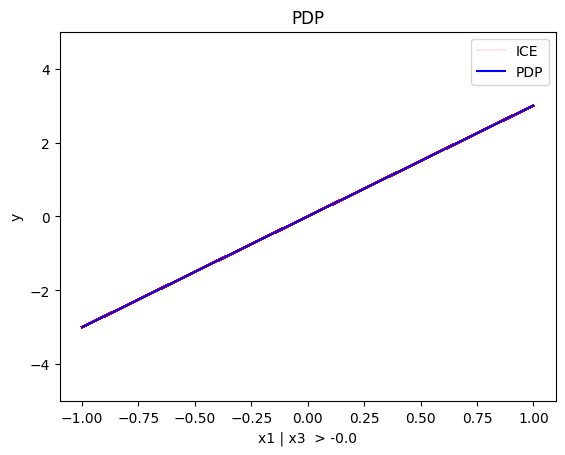
\includegraphics[width=\textwidth]{figures/simulation_1/uncor_regional_pdp_2.png}
        \caption{Regional PDP ($x_1 | x_3 > 0$)}
        \label{subfig:b}
    \end{subfigure}
    \begin{subfigure}[b]{0.33\textwidth}
        \centering
        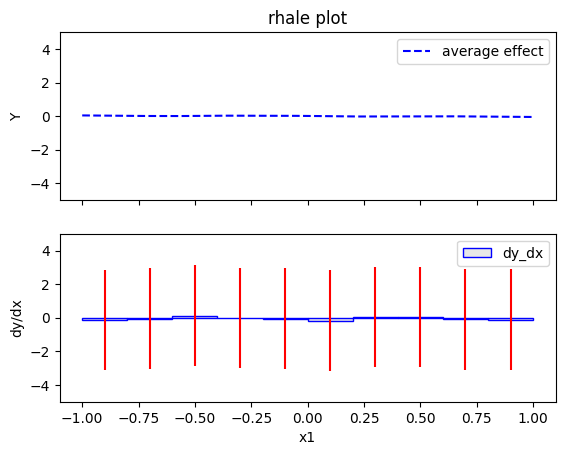
\includegraphics[width=\textwidth]{figures/simulation_1/uncor_global_rhale.png}
        \caption{Global RHALE ($x_1$)}
        \label{subfig:a}
    \end{subfigure}
    \begin{subfigure}[b]{0.33\textwidth}
        \centering
        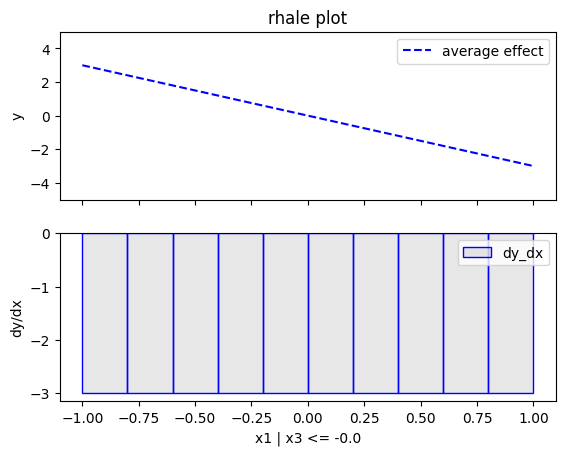
\includegraphics[width=\textwidth]{figures/simulation_1/uncor_regional_rhale_1.png}
        \caption{Regional RHALE ($x_1 | x_3 \leq 0$)}
        \label{subfig:b}
    \end{subfigure}
    \begin{subfigure}[b]{0.33\textwidth}
        \centering
        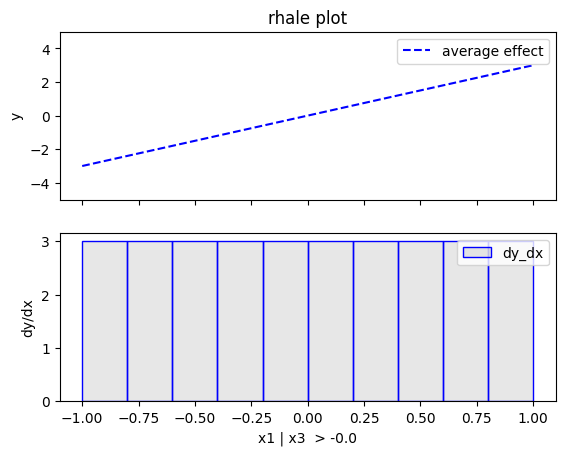
\includegraphics[width=\textwidth]{figures/simulation_1/uncor_regional_rhale_2.png}
        \caption{Regional RHALE ($x_1 | x_3 > 0$)}
        \label{subfig:b}
    \end{subfigure}
    \caption{Global and regional effect for the uncorrelated setting of synthetic example 1, using PDP and RHALE methods.}
    \label{fig:synthetic-1-uncorrelated}
  \end{figure*}

\paragraph{Correlated setting.}

  In the correlated case, due to $x_3=x_1$, the interaction terms can be written as $3x_1I_{x_1>0}$ and $-3x_1I_{x_1 \leq 0}$.
  This is because when $x_1>0$, $x_3>0$, so only the term $3x_1$ is active. Similarly, when $x_1\leq 0$, $x_3 \leq 0$, making the term $-3x_1$ active.

\begin{figure*}[t]
    \centering
    \begin{subfigure}[b]{0.49\textwidth}
        \centering
        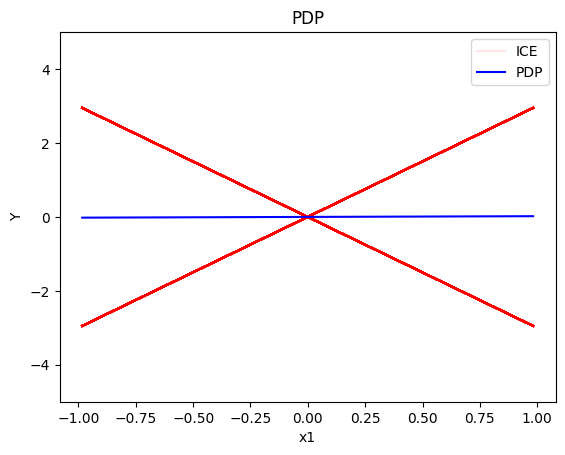
\includegraphics[width=\textwidth]{figures/simulation_1/cor_global_pdp.png}
        \caption{Global effect}
        \label{subfig:a}
    \end{subfigure}
    \begin{subfigure}[b]{0.49\textwidth}
        \centering
        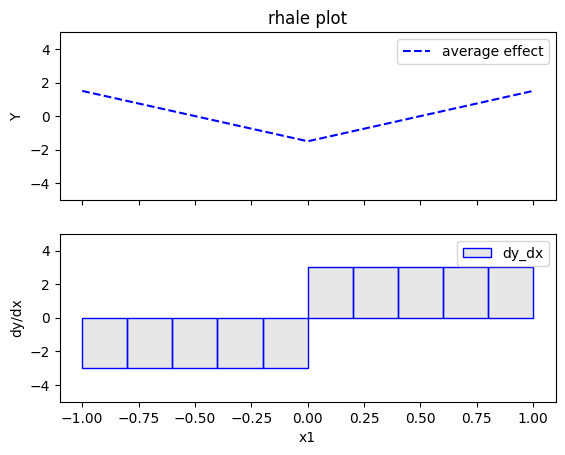
\includegraphics[width=\textwidth]{figures/simulation_1/cor_global_rhale.png}
        \caption{Global effect}
        \label{subfig:a}
    \end{subfigure}
    \caption{Global and interaction effects.}
    \label{fig:main-concept}
  \end{figure*}
  
  
\section{Conclusion and Future Work}

\bibliography{regional_rhale.bib}

\end{document}

%%
%% End of file
